%%This is a very basic article template.
%%There is just one section and two subsections.
%%This is a very basic article template.
%%There is just one section and two subsections.
\documentclass[a4paper,11pt,oneside,brazilian]{article}

\usepackage[utf8]{inputenx}
\usepackage[brazilian]{babel}
\usepackage{graphicx}
\usepackage{float}
\usepackage{textgreek}
\usepackage{mathtools}
\usepackage{enumerate}
\usepackage{xfrac}

\usepackage{multicol}

\usepackage{pgf,tikz}
\usepackage{pgfplots}
\usetikzlibrary{arrows}

\newcommand{\degre}{\ensuremath{^\circ}}
\newcommand{\bfig}{\begin{figure}[!h]\centering}
\newcommand{\efig}{\end{figure}}
\renewcommand{\thesection}{\Roman{section}} 


\definecolor{zzttqq}{rgb}{0.6,0.2,0}
\definecolor{xdxdff}{rgb}{0.49,0.49,1}
\definecolor{qqqqff}{rgb}{0,0,1}
\definecolor{cqcqcq}{rgb}{0.75,0.75,0.75}
\definecolor{uuuuuu}{rgb}{0.27,0.27,0.27}
\definecolor{uququq}{rgb}{0.25,0.25,0.25}
\definecolor{qqwuqq}{rgb}{0.0,0.39215686274509803,0.0}
\definecolor{ffqqqq}{rgb}{1.0,0.0,0.0}

 \pgfplotsset{compat=1.9}
\begin{document}

\title{Exercícios de Prática e Lógica}
\author{Prof. Eduardo Elael}
\date{Lista ENEM - PVNC 2014}
\maketitle


\begin{flushright}
  \emph{Data da realização:} 13/out/2014
\end{flushright}

\section{Matemática}
\begin{enumerate}[{R}1]
 
  \item Uma escada de $2m$ é apoiada sobre uma parede perpendicular ao chão.
  Pode-se afirmar que a distância do centro da escada ao canto, vértice entre o
  chão e a parede, é: 

  \nopagebreak[4]
  \begin{multicols}{2}
  \begin{enumerate}[a)]
    \item $0,5m$
    \item $1,0m$
    \item $1,2m$
    \item $1,5m$
  \end{enumerate}
  
	\begin{figure}[H]
		 \centering
		\begin{tikzpicture}[left, scale = 0.5, line cap=round,line
		join=round,>=triangle 45,x=1.0cm,y=1.0cm] \clip(5.76,-4.1) rectangle (12.88,4);
		\draw[color=qqwuqq,fill=qqwuqq,fill opacity=0.1] (10,-3.79) -- (9.79,-3.79) -- (9.79,-4) -- (10,-4) -- cycle;
		\draw (10,-4) -- (10,4);
		\draw [domain=5.76:10.0] plot(\x,{(--8-0*\x)/-2});
		\draw [line width=2.8pt,color=zzttqq] (10,1)-- (8,-4);
		\draw [dash pattern=on 1pt off 1pt] (9,-1.5)-- (10,-4);
		\begin{scriptsize}
		\fill [color=uququq] (9,-1.5) circle (1.5pt);
		\draw[color=uququq] (8.66,-1.18) node {$D$};
		\end{scriptsize}
		\end{tikzpicture}
	\end{figure}
  \end{multicols}
  %\nopagebreak[4]
  \item Um rolo de pintar composto por um cilindro de $10cm$ de diâmetro é
  inserido diagonalmente no vaso de tinta, a fim de fazer um detalhe ondulado na
  pintura (como mostra a figura). O rolo é passado por uma superficie plana
  para formar esse detalhe. Nessa situação o espaçamento entre dois vales
  consecutivos da ondulação criada é:
  

  \nopagebreak[4]

	\begin{figure}[H]
		 \centering
		 \includegraphics[width=1\columnwidth]{../rolo.jpg}
		 %\caption{Tubo da eletrônica embarcada}
		 \label{fig:rolo}
	 \end{figure}
	 
  \pagebreak[4]
  \begin{enumerate}[a)]
    \item $10\pi cm$
    \item $20\pi cm$
    \item $50\pi cm$
    \item $100\pi cm$
  \end{enumerate}
		
  %\pagebreak[4]
  \item Um cubo é equilibrado sobre apenas um de seus vértices. Quando visto de
  cima ele se apresenta como um hexagono regular de lado de $1 cm$ de lado
  (vide figuras). Para isso a superfície do cubo deve ser de:

  \nopagebreak[4]
  \begin{multicols}{2}
  
	\begin{figure}[H]
		 \centering
		 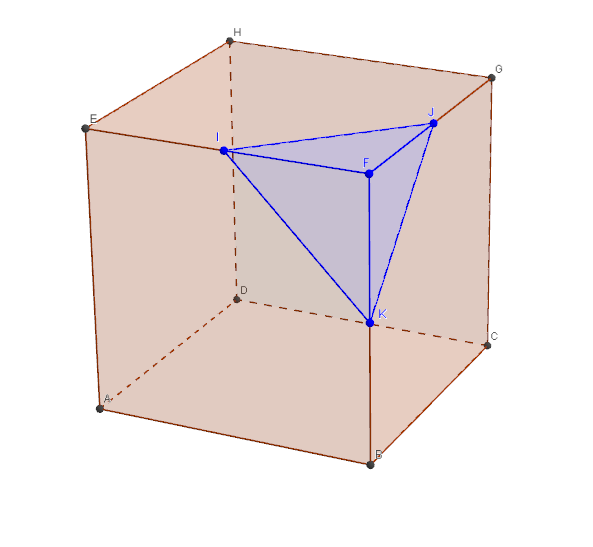
\includegraphics[width=1\columnwidth]{../cube.jpg}
		 %\caption{Tubo da eletrônica embarcada}
		 \label{fig:cube}
	\end{figure}
	
	\begin{figure}[H]
		 \centering
			\begin{tikzpicture}[ line cap=round,line join=round,>=triangle
			45,x=1.0cm,y=1.0cm] \clip(6.38,-5.78) rectangle (11.56,-0.66);
			\fill[color=zzttqq,fill=zzttqq,fill opacity=0.1] (8,-5) -- (10,-5) -- (11,-3.27) -- (10,-1.54) -- (8,-1.54) -- (7,-3.27) -- cycle;
			\draw [line width=1.2pt,color=zzttqq] (8,-5)-- (10,-5);
			\draw [line width=1.2pt,color=zzttqq] (10,-5)-- (11,-3.27);
			\draw [line width=1.2pt,color=zzttqq] (11,-3.27)-- (10,-1.54);
			\draw [line width=1.2pt,color=zzttqq] (10,-1.54)-- (8,-1.54);
			\draw [line width=1.2pt,color=zzttqq] (8,-1.54)-- (7,-3.27);
			\draw [line width=1.2pt,color=zzttqq] (7,-3.27)-- (8,-5);
			\draw [line width=1.2pt] (8,-1.54)-- (9,-3.27);
			\draw [line width=1.2pt] (9,-3.27)-- (11,-3.27);
			\draw [line width=1.2pt] (9,-3.27)-- (8,-5);
			\draw [line width=0.4pt,dash pattern=on 1pt off 1pt] (10,-1.54)-- (9,-3.27);
			\draw [line width=0.4pt,dash pattern=on 1pt off 1pt] (9,-3.27)-- (7,-3.27);
			\draw [line width=0.4pt,dash pattern=on 1pt off 1pt] (9,-3.27)-- (10,-5);
			\draw (8.66,-0.78) node[anchor=north west] {$$1 cm$$};
			\end{tikzpicture}
	\end{figure}
  \end{multicols}
  
  \begin{enumerate}[a)]
    \item $12 cm^2$
    \item $9 cm^2$
    \item $6 cm^2$
    \item $2 cm^2$
  \end{enumerate}

  \item Uma balança de cozinha funciona encontrando o ponto de equilíbrio entre
  o ingrediente a ser medido e um peso conhecido. Para encontrar o ponto de
  equilibrio move-se a base sobre o qual a balança se equilibra, vide figura,
  em seguida deve-se olhar qual o valor em gramas que a base está apontando. 
  
  \begin{multicols}{2}
  
	\begin{figure}[H]
		 \centering
		 \includegraphics[width=0.9\columnwidth]{../balanca01PB.jpg}
		 %\caption{Tubo da eletrônica embarcada}
		 \label{fig:bal01}
	\end{figure}
  \nopagebreak[4]
	

	\begin{figure}[H]
		 \centering
		 \includegraphics[width=0.95\columnwidth]{../balanca02PB.jpg}
		 %\caption{Tubo da eletrônica embarcada}
		 \label{fig:bal02}
	\end{figure}
  \end{multicols}
  
  O princípio da balança funciona, pois existe uma relação entre a distância que
  se desloca o ponto de equilíbrio e o peso do ingrediente que está sendo
  medido. Esse deslocamento é medido a partir do zero, onde não há ingrediente
  sendo medido. O gráfico que melhor esboça a relação entre a distância que o
  ponto de equilíbrio é deslocado e o peso do ingrediente sendo medido é:
  
  \begin{enumerate}[a)]
    \item 
  \begin{tikzpicture}
    \begin{axis}[
        ymin=0,ymax=125,
        xmin=0,xmax=14,
        ticks=none,axis x line=bottom,axis y line=left,ylabel={Peso }, xlabel={Distância},
    ]
    \addplot[
        domain=0:249.999,
        samples=1000,
    ]
        { (15/(15-x)-1)*10};
    \end{axis}
\end{tikzpicture}
    \item 


  \begin{tikzpicture}
    \begin{axis}[
        ymin=0,ymax=150,
        xmin=0,xmax=14,
        ticks=none,axis x line=bottom,axis y line=left,ylabel={Peso},
        xlabel={Distância}, ]
    \addplot[
        domain=0:249.999,
        samples=1000,
    ]
        { (15-15/(1+x))*10};
    \end{axis}
\end{tikzpicture}
    \item 

  \begin{tikzpicture}
    \begin{axis}[
        ymin=0,ymax=14,
        xmin=0,xmax=14,
        ticks=none,axis x line=bottom,axis y line=left,ylabel={Peso}, xlabel={Distância},
    ]
    \addplot[
        domain=0:249.999,
        samples=1000,
    ]
        { x};
    \end{axis}
\end{tikzpicture}
    \item 

  \begin{tikzpicture}
    \begin{axis}[
        ymin=0,ymax=1.2,
        xmin=0,xmax=180,
        ticks=none,axis x line=bottom,axis y line=left,ylabel={Peso }, xlabel={Distância},
    ]
    \addplot[
        domain=0:249.999,
        samples=1000,
    ]
        { sin(x)};
    \end{axis}
\end{tikzpicture}
\end{enumerate}
\end{enumerate}

\end{document}
